\begin{figure}
%%% trim = left, bottom, right, top
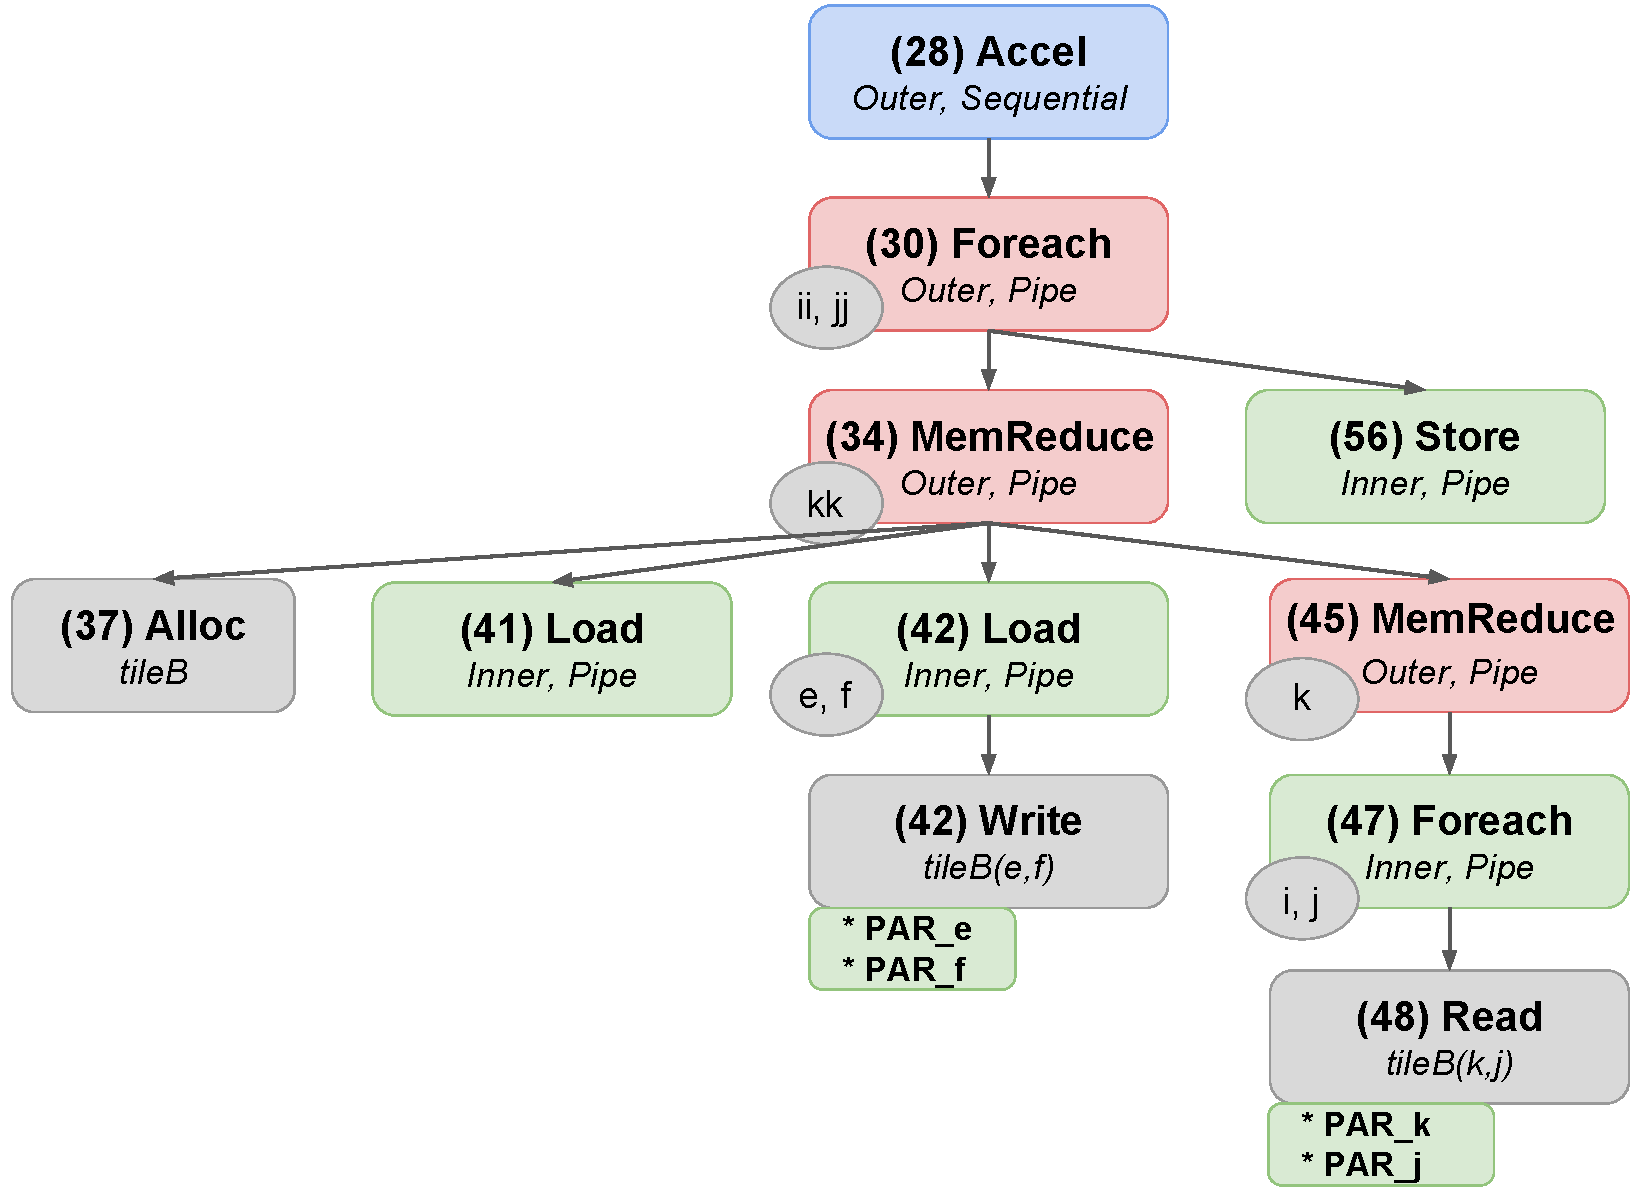
\includegraphics[clip, width=0.9\columnwidth]{figs/control_tree_gemm.pdf}
\vspace{-10pt}
\caption{The control/access tree for the \texttt{\small{SRAM tileB}} in the matrix multiply example in Figure~\ref{fig:matmult}.
%Control nodes are annotated with their level (outer versus inner), schedule, and loop iterator name. Memory access nodes are annotated with their parallelization factor.
\vspace{-5pt}
}
\label{fig:controlTree}
\end{figure}

\section{Intermediate Representation}

Spatial programs are internally represented in the compiler as a hierarchical dataflow graph (DFG).
Nodes in this graph represent control structures, data operations, and memory allocations, while edges represent data and effect dependencies.
Nesting of controllers directly translates to the hierarchy in the intermediate representation.
Design parameters are kept as graph metadata, such that they can be independently updated without changing the graph itself.


When discussing DFG transformations and optimizations, it is often useful to think about the graph as a controller/access tree. Figure~\ref{fig:controlTree} shows an example of one such controller tree for the memory {\texttt{\small{tileB}} in the Spatial code example in Figure~\ref{fig:matmult}. Note that transfers between on-chip and off-chip memory expand to a control node which linearly accesses the on-chip memory, in this case by iterators \texttt{e} and \texttt{f}.
This tree abstracts away most primitive operations, leaving only relevant controller hierarchy and the memory
accesses for a specific memory.


Within the acceleratable subset of Spatial, nodes are formally separated into three categories:
control nodes, memory allocation nodes, and primitive nodes.
Control nodes represent state machine structures like \texttt{\small{Foreach}} and \texttt{\small{Reduce}} described in Section~\ref{controls}.
Primitive nodes are operations which may consume, but never produce, control signals, including on-chip memory accesses.
Primitive nodes are further broken down into ``physical'' operations requiring resources and ``ephemeral'' operations which are only used for bookkeeping purposes in the compiler. For example, bit selects and grouping of words into structs require no hardware resources but are used to track necessary wires in the generated code.
